%*******************************************************************************
%****************************** Fourth Chapter *********************************
%*******************************************************************************

\chapter{Characterisation of III-Nitride Microdisk Cavities}

\ifpdf
    \graphicspath{{Chapter2/Figs/Raster/}{Chapter2/Figs/PDF/}{Chapter2/Figs/}}
\else
    \graphicspath{{Chapter2/Figs/Vector/}{Chapter2/Figs/}}
\fi


\section[Short title]{Background}

Microcavities possess particular optical properties, as discussed in section \ref{cavity section}. Strongly-coupled cavities are crucial in accomplishing important quantum information processing tasks such as controlled coherent coupling and the entanglement of quantum systems \cite{Hennessy2007}. Weakly-coupled microcavity systems have many applications in optoelectronic devices such as high efficiency, low threshold lasers \cite{Vahala2003}. Applications for both strong and weak coupling cavities are discussed in more detail in section \ref{cavity section}.
\\ Though various geometries for cavities exist, in this chapter we will specifically address III-nitride microdisk cavities. Microdisk III-nitride cavities have presented several challenges in terms of fabrication, due to chemical and thermal properties of GaN discussed in section \ref{microdisk section}. Currently, one of the preferred methods of for the fabrication of III-nitride microdisk cavities is PEC etching of an InGaN sacrificial superlattice \nomenclature[z-SSL]{SSL}{Sacrificial Superlattice} (SSL) \cite{Puchtler2015}. This in itself presents issues, as El-Ella \textit{et al.} have shown that the growth of the InGaN SSL with a quantum dot (QD) layer can introduce dislocations into the structure \cite{El-Ella2011a}. Furthermore, PEC etching can be a difficult process to control as it is heavily dependent on conductivity and hence can be defect-selective \cite{Visconti2001,Youtsey1999,Youtsey1998} and dopant-selective \cite{Youtsey1999}, occasionally resulting in protrusions or roughness \cite{Puchtler2015} on the etched underside of microdisk cavities. The work contained in this chapter is a microscopy-based investigation into fabrication issues in GaN/InGaN microdisk cavities.

\subsection{PEC etching}

\label{microdisk fab section}
As discussed in section \ref{microdisk section}, the ability to perform an effective 'undercut' is a crucial aspect in the fabrication of III-nitride microcavities. PEC etching is a commonly used technique to achieve an undercut microdisk and will be introduced here.
PEC etching was first reported in III-nitrides by Minsky \textit{et al.} \cite{Minsky1996}, and is an extremely effective method to perform selective etching as it can be defect-selective and bandgap-selective. To achieve an undercut on a III-nitride microdisk the following set-up is typically used: a GaN filter is used to absorb light emitted by a Xenon lamp, allowing light of wavelength longer than ~360nm to interact with the structure thus ensuring the majority of carriers are generated in the sacrificial InGaN layer. Holes generated by the incident light diffuse toward the surface of the InGaN layer which in this case acts as an anode whilst the electrons diffuse toward to the metal cathode due to both the overall potential in the connected cell and the band-bending occurring at the surfaces. This process is shown schematically in Fig.\ref{PECetch}.

\begin{figure}[h]
	\centering
	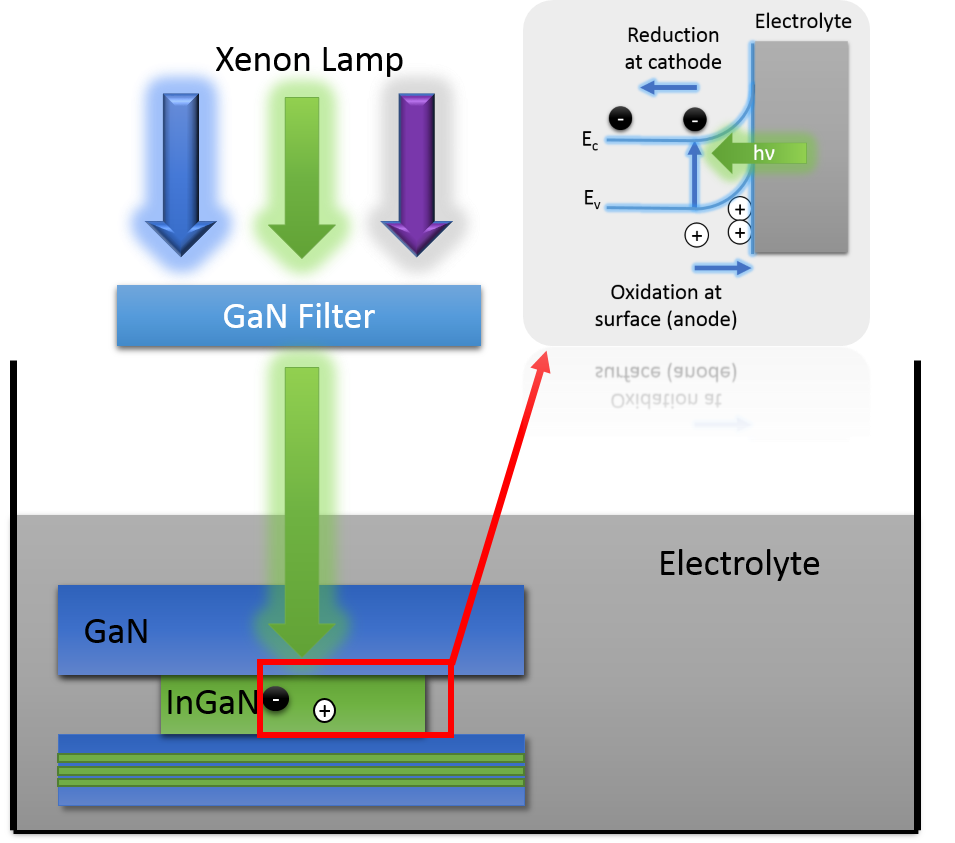
\includegraphics[width=0.8\textwidth]{Figs/Ch4/PEC.png}
	\caption {PEC etching set-up, with the charge transfer process shown in the inset.}
	\label{PECetch}
\end{figure}
\FloatBarrier 

The excess concentration of holes at the sacrificial layer surface drives the oxidation of InGaN, forming Ga2O3, In2O3 and N2, while at the cathode a reduction process is driven by the excess electrons. The oxide generated by the reduction process is then dissolved in the electrolyte, thus etching the sacrificial layer. It is clear that the etch rate of the sacrificial layer is governed by several factors: the rate of generation of the photo-generated electron hole pairs, their diffusion rates towards the anode or cathode, and the concentration of the electrolyte (HCl in this case). It is due to this photo-generated carrier concentration dependence that the PEC etching process is defect and dopant selective.

\subsection{Whisker Generation in PEC Etching}
Youtsey \textit{et al.} demonstrated the ability of dislocations to hinder the progress of PEC etching and used this to determine the dislocation density of n-type GaN films. Unetched material (or ‘whiskers’) remained at dislocation sites after the PEC etching process due to the electrically active nature of dislocations in GaN, as shown in Fig. \ref{PECwhiskeryoutsey}.

\begin{figure}[h]
 	\centering
 	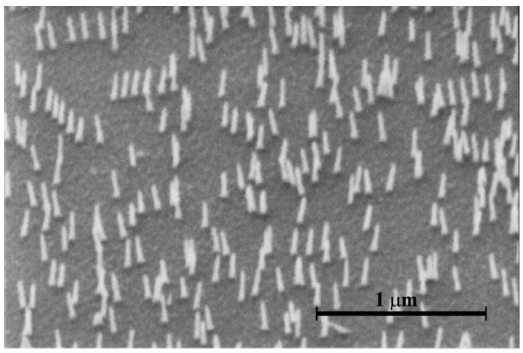
\includegraphics[width=0.8\textwidth]{Figs/Ch4/youtseywhisker.png}
 	\caption {SEM image of whiskers produced by etching of dislocations in an MOCVD GaN film grown on a silicon carbide (SiC) substrate. Reproduced from \cite{Youtsey1999}}
 	\label{PECwhiskeryoutsey}
\end{figure}
\FloatBarrier 

It was confirmed through cross-sectional TEM that both mixed and edge dislocations result in the formation of whiskers \cite{Youtsey1998}.\\
The mechanism through which the presence of dislocations impedes the PEC etching process relates to the charge trapping property of TDs: it has been suggested based on cathodoluminescence (CL) studies that TDs act as non-radiative recombination centres, as mentioned in section \ref{dislocation section}. In this case, photogenerated holes in the vicinity of TDs would be prevented from diffusing to the epilayer surface thus resulting in unetched material. There is also evidence for negatively charged TDs in n-type GaN \cite{Cherns2000}, which could lead to hole-trapping at TDs presenting an alternative or additional explanation for the reduction in surface hole concentration and thus reduced etch rate in areas adjacent to TDs \cite{Youtsey1998}.

\subsection{Q-factor Reduction in Microdisks}

El-Ella \textit{et al.} first demonstrated the effect of dislocations on the Q-factor of GaN microdisks containing an InGaN QD active layer. By carefully controlling the In compostion of the SSL, the authors were able to produce two sets of microdisks, one with a dislocation density of $3 \times 10^{9} cm^{-2}$ (sample A) and the other with a lower density of $7 \times 10^{8} cm^{-2}$ (sample B). As expected, microdisks fabricated from sample A exhibited a larger density of whiskers on the underside of the disk. SEM was used to establish that 90$\%$ of disks fabricated from material A exhibited whiskers, compared to only 20$\%$  of disks fabricated from structure B. The difference between the two samples in terms of Q-factor is illustrated in Fig.\ref{El-Ellacomp} which includes data for eight microdisks fabricated from each sample. 

\begin{figure}[h]
	\centering
	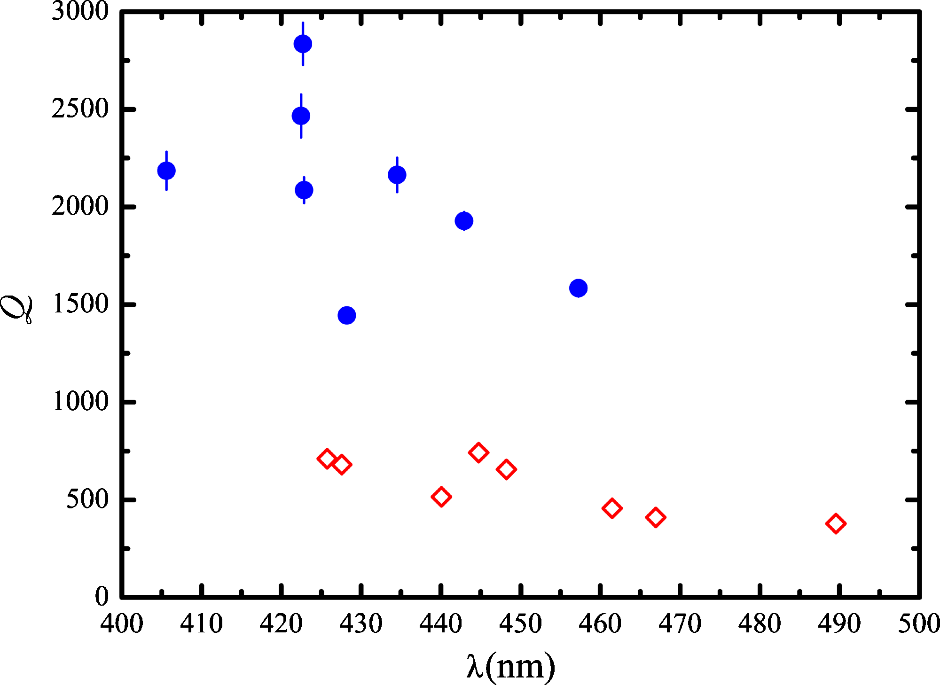
\includegraphics[width=0.8\textwidth]{Figs/Ch4/elellacomp.png}
	\caption {Q values from eight modes of microdisks fabricated from structure A(\textcolor{red}{$\lozenge$}) and B ((\textcolor{blue}{$\Bigcdot$}). Reproduced from \cite{El-Ella2011}.}
	\label{El-Ellacomp}
\end{figure}
\FloatBarrier 

All microdisks fabricated from sample B show a larger Q-factor than all microdisks from sample A. The average Q-factors for microdisks fabricated from samples A and B were 600 and 2000 respectively, suggesting a strong correlation between Q-factor and dislocation density \cite{El-Ella2011}.\\
Puchtler \textit{et al.} addressed these issues by identifying not only the number but also the position of TDs in individual microdisk cavities and evaluating the effect of these parameters on microdisk Q-factors\cite{Puchtler2015}.  Unlike the study by El-Ella \textit{et al.}, this work correlated the performance of each individual device structure with its specific structure. In this study, dark spots in CL images (arising from non-radiative recombination as discussed in section \ref{dislocation section}) were used as a signature for the presence of dislocations, and hence whiskers.  The authors established the correspondence of dark spots in the CL to whiskers by comparing plan-view panchromatic CL images with side-view SEM images of the microdisks. The results of these correlative measurements are shown in Fig.\ref{puchtlerdislocation}.

\begin{figure}[h]
	\centering
	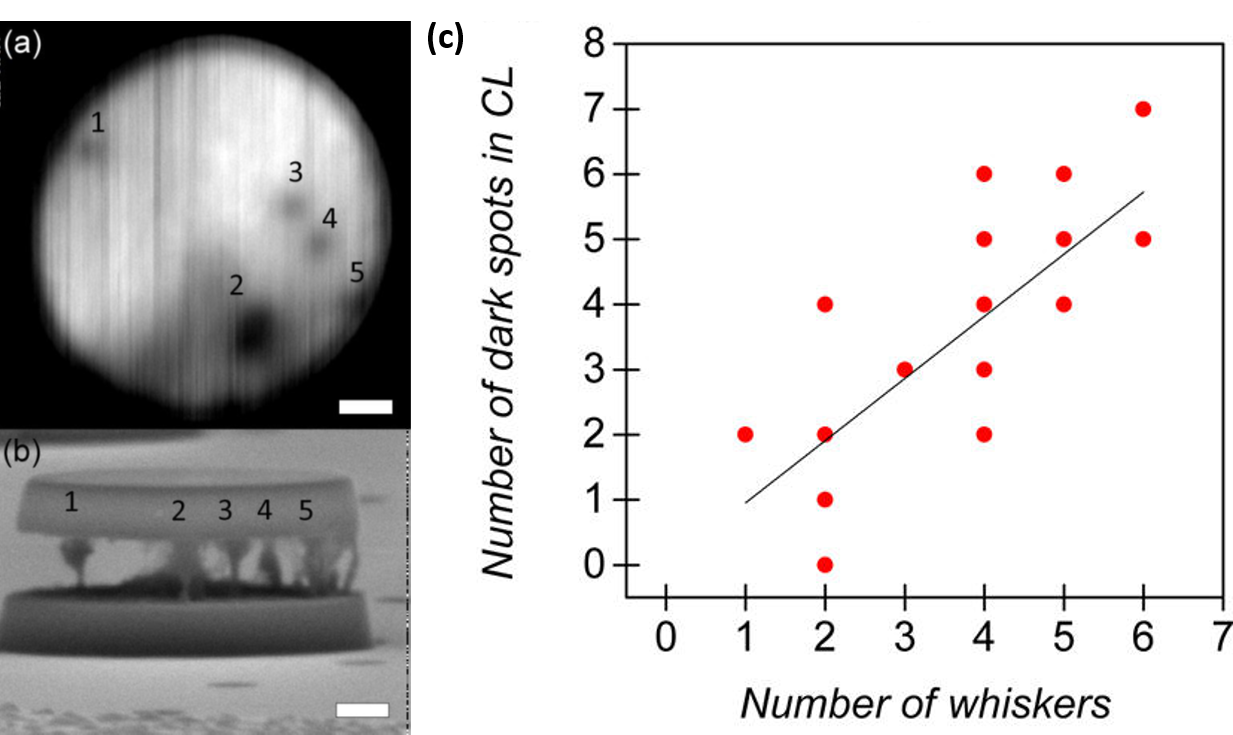
\includegraphics[width=1\textwidth]{Figs/Ch4/puchtlerdislocation.png}
	\caption {a) Sample plan-view CL b) Corresponding side-view SEM image of an undercut microdisk with whiskers corresponding to the dark spots shown in a). c) Relationship between whiskers on the underside and dark features counted in plan-view CL. Adapted from \cite{Puchtler2015}.}
	\label{puchtlerdislocation}
\end{figure}
\FloatBarrier 
